\documentclass{article}

\PassOptionsToPackage{round, sort&compress}{natbib}

\usepackage{neurips_2026}
% \usepackage[preprint]{neurips_2026}
% \usepackage[final]{neurips_2026}

\usepackage[utf8]{inputenc}
\usepackage[T1]{fontenc}
\usepackage{hyperref}
\usepackage{url}
\usepackage{booktabs}
\usepackage{amsmath, amssymb, amsthm, amsfonts}
\usepackage{mathtools}
\usepackage{bbm}
\usepackage{nicefrac}
\usepackage{microtype}
\usepackage{xcolor}
\usepackage{graphicx}
\usepackage{subcaption}

\definecolor{DarkBlue}{RGB}{0,45,130}
\hypersetup{
  colorlinks=true,
  linkcolor=DarkBlue,
  citecolor=DarkBlue,
  urlcolor=DarkBlue
}
\setcitestyle{round,sort&compress}

% Theorem environments
\newtheorem{theorem}{Theorem}
\newtheorem{lemma}[theorem]{Lemma}
\newtheorem{proposition}[theorem]{Proposition}
\newtheorem{corollary}[theorem]{Corollary}
\newtheorem{definition}[theorem]{Definition}
\newtheorem{remark}[theorem]{Remark}
\newtheorem{assumption}[theorem]{Assumption}

% Math macros
\DeclareMathOperator*{\argmin}{arg\,min}
\DeclareMathOperator*{\argmax}{arg\,max}
\DeclareMathOperator{\softplus}{softplus}
\newcommand{\R}{\mathbb{R}}
\newcommand{\E}{\mathbb{E}}
\renewcommand{\Pr}{\mathbb{P}}
\newcommand{\Xcal}{\mathcal{X}}
\newcommand{\Ycal}{\mathcal{Y}}
\newcommand{\Acal}{\mathcal{A}}
\newcommand{\Dcal}{\mathcal{D}}
\newcommand{\Ecal}{\mathcal{E}}
\newcommand{\Hcal}{\mathcal{H}}
\newcommand{\Lcal}{\mathcal{L}}
\newcommand{\Rcal}{\mathcal{R}}
\newcommand{\Ncal}{\mathcal{N}}
\newcommand{\TV}{\mathrm{TV}}
\newcommand{\KL}{\mathrm{KL}}
\newcommand{\ind}{\mathbbm{1}}
\newcommand{\defer}{\bot}

\title{Learning to Abstain for Reliable Physics-Informed Neural Networks}

\author{%
  Anonymous Author(s) \\
  Affiliation \\
  Address \\
  \texttt{email}
}

\begin{document}

\maketitle

\begin{abstract}
Physics-informed neural networks (PINNs) provide cheap, mesh-free,
differentiable surrogates for partial differential equations, but their
pointwise accuracy is known to be \emph{spatially non-uniform}: a small
subdomain typically carries a disproportionate share of the error. Existing
remedies---adaptive sampling, loss reweighting, causal training, domain
decomposition---rebalance the optimisation but still return a single global
predictor that the user must trust everywhere. We argue instead for
\emph{learning with abstention}: a frozen PINN is paired with a classical
solver, and a learned rejector decides at each spatial location whether to
commit to the PINN prediction or to abstain to the solver. We cast this as
a regression abstention problem with an input-dependent cost derived from
the PDE residual and a linearised error-transport estimate, derive its
Bayes-optimal rejector, and design a consistent surrogate for the
predictor--rejector formulation extended from a categorical predictor with
$0$--$1$ loss to a continuous predictor with a non-negative discrepancy.
We prove an $\Hcal$-consistency bound for the proposed surrogate and show
that the induced hybrid solution inherits a controllable PDE error from
the rejection decisions.

\end{abstract}

\section{Introduction}
\label{sec:intro}

Physics-informed neural networks (PINNs) are a widely used deep-learning
surrogate for partial differential equations
\citep{raissi2019physics,karniadakis2021physics,cuomo2022scientific,
lu2021deepxde}. Their appeal is clearest after training: a neural network
represents a mesh-free, differentiable field that can be evaluated at
arbitrary spatial or space-time locations without running a new global
linear or nonlinear solve \citep{leveque2007finite,brenner2008mathematical}.
This amortised evaluation cost is attractive, but it does not by itself
provide the local accuracy guarantees expected of a resolved numerical
discretisation. On several standard PDE benchmarks, PINNs can exhibit large
errors in regimes with multiscale structure, stiffness, sharp gradients, or
unbalanced residual terms \citep{krishnapriyan2021,wang2022whenpinns,
wang2021understanding}. Existing a-posteriori analyses relate residual
norms to global solution errors under stability and approximation
assumptions \citep{mishra2022estimates}; such bounds are valuable, but they
do not directly identify the particular points or subregions where a trained
PINN should be trusted.

The missing object is therefore a \emph{local trust rule}. Empirically, PINN
errors are often highly non-uniform over the domain: a model may approximate
large smooth regions well while failing near fronts, boundary layers,
singular features, or other regions whose solution components are difficult
for the training dynamics to capture \citep{krishnapriyan2021,
wang2022whenpinns,wang2022respecting}. This observation suggests a different
deployment goal from uniform replacement of a classical solver. Instead of
asking a single trained PINN to be accurate everywhere, we ask it to predict
where it is accurate enough to use and where it should abstain. The natural
statistical language for this goal is learning with abstention
\citep{chow1970,bartlett2008classification,Geifman_El-Yaniv_2017,cortes,
cortes2024theory,cao2022generalizing,ni2019calibration,Mao_Mohri_Zhong_2023,
theoretically}: a predictor is paired with a rejector that decides, for each
input, whether to return the prediction or abstain.

Classical abstention would return only a rejection symbol $\bot$ on rejected
inputs. For PDE surrogates this is usually not enough, because downstream
simulation, visualisation, or physical diagnostics often require a complete
solution field. We therefore study abstention with a fallback solver: a
frozen PINN $\widehat{u}_\theta$ supplies the field on accepted points, while
a classical numerical solver is used on rejected regions or queried
locations. If the rejector abstains on a small fraction of the domain, the
hybrid can preserve much of the amortised efficiency of the PINN while using
the solver where the PINN is estimated to be unreliable. The precise cost
depends on the implementation of the fallback solve and the geometry of the
rejected set, so we model it abstractly through an input-dependent
abstention cost $c(x)$ rather than assuming a universal per-point solver
cost.

This perspective is complementary to the large body of work that improves
PINN training. Loss reweighting based on gradient-flow or neural-tangent
kernel diagnostics \citep{wang2021understanding,wang2022whenpinns},
self-adaptive collocation weights \citep{mcclenny2023self}, causal
residual training \citep{wang2022respecting}, residual-based adaptive
sampling \citep{wu2023comprehensive,daw2023mitigating}, and domain
decomposition methods \citep{jagtap2020extended,jagtap2020conservative,
moseley2023finite} can substantially improve particular classes of PDE
problems. However, they still return a single global predictor. They do not,
by themselves, convert a trained PINN into a pointwise certificate of
reliability, nor do they give a post-hoc rule for routing an already-trained
model to a fallback solver. Our goal is to add precisely that missing layer:
a learned rejector whose decision is calibrated to the local error of a
fixed PINN relative to the cost of abstention.

In the setting studied here, the trained PINN is fixed and the learned object
is only the rejector. We write the fixed predictor as
$h=\widehat{u}_\theta$ and measure its pointwise error through a
non-negative discrepancy $\psi(h(x),u^\star(x))$. The ideal rejection rule
compares the conditional risk
$\eta_h(x)=\E[\psi(h(x),Y)\mid X=x]$ with an abstention cost $c(x)$:
accept the PINN when $\eta_h(x)\le c(x)$ and abstain otherwise. This is the
same structural comparison as classical rejection, but in a continuous
regression setting with a spatially varying cost. In practice, $\eta_h$ is
unobserved, so the rejector must be trained from computable local signals
such as the PDE residual and linearised error-transport estimates. The
theoretical task is therefore to design a smooth surrogate whose minimisation
learns the same accept--reject decision as the Bayes rule.

\paragraph{Contributions.}
\begin{itemize}
\item We introduce a post-hoc abstention layer for PINNs: a trained field
  $\widehat{u}_\theta$ is kept frozen, and a separate rejector learns the
  subregions on which the PINN should be replaced by a numerical fallback.
\item We formulate this layer as regression with rejection for continuous
  solution fields, with a general discrepancy $\psi$ and an
  input-dependent abstention cost $c(x)$, rather than the constant-cost
  classification setting usually considered in abstention.
\item We identify the Bayes rejector for a fixed PINN as the local threshold
  rule $\eta_h(x)>c(x)$, where
  $\eta_h(x)=\E[\psi(h(x),Y)\mid X=x]$, making explicit the quantity that a
  PINN reliability model must approximate.
\item We design the rejector around computable physics-based signals,
  combining strong-form residual information with linearised
  error-transport estimates to target the local residual--error gap.
\item We provide the surrogate-consistency and hybrid-solution analysis
  needed for deployment: minimising the smooth rejector loss controls the
  hard abstention decision, and the solver-filled regions yield a complete
  PDE field rather than a rejection symbol.
\end{itemize}

%\section{Related Work}
%\label{sec:related}
%
%\paragraph{Learning with abstention.} The rejection option originates with
%\citet{chow1970}, who characterised the optimal error--reject trade-off in
%classification. Subsequent work developed convex and calibrated losses for
%binary classification with rejection \citep{bartlett2008classification,
%cortes,cortes2024theory}, selective deep classification
%\citep{Geifman_El-Yaniv_2017}, and multi-class rejection
%\citep{ni2019calibration,cao2022generalizing}. The predictor--rejector
%formulation most closely related to ours is that of
%\citet{Mao_Mohri_Zhong_2023}, together with score-based abstention losses
%analysed by \citet{theoretically}. Regression with cost-based rejection was
%formalised by \citet{cheng2023regression}. Our setting differs in two
%respects: the fixed predictor is a PDE solution field evaluated over a
%spatial or space-time domain, and the abstention cost is tied to the local
%value of invoking a numerical fallback rather than to a constant reject
%penalty.
%
%\paragraph{Learning to defer.} A neighbouring literature routes examples to
%external experts instead of returning a pure abstention decision
%\citep{madras2018predict,mozannar2021consistent,Verma2022LearningTD,
%Cao_Mozannar_Feng_Wei_An_2023,mao2023twostage,
%mao2024principledapproacheslearningdefer,liu2026more}. Recent variants
%consider regression \citep{mao2024regressionmultiexpertdeferral},
%multi-task settings \citep{montreuil2024twostagelearningtodefermultitasklearning},
%top-$k$ expert routing \citep{montreuil2026why}, online or budgeted experts
%\citep{desalvo2025budgetedmultipleexpertdeferral}, and non-stationary
%streams \citep{montreuil2026learning}. Our fallback solver can be viewed as
%a single expert with known numerical role and cost model. We use abstention
%terminology because the learned decision is binary for a fixed PINN: use the
%PINN prediction or reject it in favour of the solver.
%
%\paragraph{$\Hcal$-consistency.} Classical consistency asks whether
%minimising a surrogate risk also minimises the target risk in the large-data
%limit \citep{bartlett2006convexity,tewari2007consistency,Steinwart2007HowTC,
%Zhang}. $\Hcal$-consistency gives sharper, hypothesis-class-specific excess
%risk bounds and has been developed for multi-class learning, adversarial
%robustness, abstention, and deferral
%\citep{Awasthi_Mao_Mohri_Zhong_2022_multi,mao2024h,
%mao2023crossentropylossfunctionstheoretical,mao2024universalgrowth,
%mao2024realizablehconsistentbayesconsistentloss}. We use this viewpoint to
%ask whether a smooth surrogate for the rejector controls the excess
%abstention risk within the chosen rejector class.
%
%\paragraph{Physics-informed neural networks.} PINNs were introduced by
%\citet{raissi2019physics} and are surveyed in
%\citet{karniadakis2021physics,cuomo2022scientific}. Their optimisation and
%generalisation failure modes have been studied through gradient-flow,
%neural-tangent-kernel, stiffness, and propagation analyses
%\citep{wang2021understanding,wang2022whenpinns,krishnapriyan2021,
%wang2022respecting}. Practical remedies include adaptive loss weighting
%\citep{mcclenny2023self}, adaptive or residual-based collocation sampling
%\citep{wu2023comprehensive,daw2023mitigating}, and domain decomposition
%\citep{jagtap2020extended,jagtap2020conservative,moseley2023finite}.
%\citet{mishra2022estimates} provide a-posteriori estimates connecting
%residual norms with global solution error under stability assumptions. These
%methods improve training or global error control; our contribution is
%post-hoc and local, learning when an already-trained PINN should be trusted.

\section{Background}
\label{sec:prelim}

We define for the rest of the paper: learning to
reject for a fixed regression rule (Section~\ref{sec:bg-reject}) and the
standard PINN formulation for PDEs (Section~\ref{sec:bg-pinn}).

\subsection{Learning to reject in regression}
\label{sec:bg-reject}

Let $(X,Y)$ be a random pair with joint distribution $\Dcal$ on
$\Xcal \times \Ycal$, where $\Xcal \subseteq \R^{d_x}$ is a measurable
input space and $\Ycal \subseteq \R^{d_u}$ is a measurable response space.
Throughout,
$\psi:\Ycal\times\Ycal\to\R_{\geq 0}$ denotes a measurable non-negative
discrepancy, such as the squared loss
$\psi(a,b)=\tfrac{1}{2}\|a-b\|_2^2$; boundedness of $\psi$ is assumed only
when it is required by a stated consistency bound.

A regression rule with rejection is a pair $(h,r)$ in which
$h:\Xcal\to\Ycal$ is a measurable predictor and
$r:\Xcal\to\{0,1\}$ is a measurable rejector. We use the convention
$r(x)=0$ to accept the prediction $h(x)$ and $r(x)=1$ to abstain. Following
the classical rejection literature, abstention trades prediction error
against a rejection cost \citep{chow1970,bartlett2008classification,
cortes,cortes2024theory}. Most standard formulations take this cost to be
constant, i.e.\ $c(x)\equiv c$ \citep{chow1970,
bartlett2008classification,Geifman_El-Yaniv_2017,ni2019calibration,
cao2022generalizing,Mao_Mohri_Zhong_2023}; we write
$c:\Xcal\to[0,C]$ to allow the more general input-dependent case, expressed
in the same units as $\psi$. We work in a second-stage
predictor--rejector setting \citep{cortes,Mao_Mohri_Zhong_2023,
cheng2023regression}, where $h$ is fixed and only $r$ is learned. The
pointwise loss is
\begin{equation}
  \ell_{\mathrm{abs}}\bigl(h,r;\,x,y\bigr)
  :=
  \psi\bigl(h(x),y\bigr)\ind\{r(x)=0\}
  +
  c(x)\ind\{r(x)=1\},
  \label{eq:abs-loss}
\end{equation}
with population risk
$\Ecal_{\ell_{\mathrm{abs}}}(h,r)
:=\E_{(X,Y)\sim\Dcal}[\ell_{\mathrm{abs}}(h,r;\,X,Y)]$. When the rule
accepts, it pays the discrepancy of the fixed predictor; when it abstains,
it pays $c(X)$.

\begin{lemma}[Bayes-optimal rejector]
\label{lem:bayes-rej}
For a fixed predictor $h$, define
$\eta_h(x):=\E[\psi(h(x),Y)\mid X=x]$. Then, for $\Pr_X$-a.e.\ $x$, the
Bayes-optimal rejector is
\[
  r^\star(x) \in
  \begin{cases}
    \{0\}, & \eta_h(x) \leq c(x),\\
    \{1\}, & \eta_h(x) > c(x),
  \end{cases}
\]
where $r^\star(x)=0$ accepts $h(x)$ and $r^\star(x)=1$ abstains.
\end{lemma}

The proof is the pointwise comparison of the two available costs,
$\eta_h(x)$ and $c(x)$. Thus the rejector only needs to learn the sign of
$\eta_h(x)-c(x)$. We use a measurable score $s:\Xcal\to\R$ from a rejector
class $\Hcal_r$ and define $r_s(x):=\ind\{s(x)>0\}$. A smooth surrogate
$\Phi_{\mathrm{abs}}$ for the discontinuous loss
\eqref{eq:abs-loss} is useful only if small surrogate excess risk controls
the true abstention excess risk in $\Hcal_r$, in the sense of
$\Hcal$-consistency bounds
\citep{Awasthi_Mao_Mohri_Zhong_2022_multi,
mao2023crossentropylossfunctionstheoretical,Mao_Mohri_Zhong_2023}. This
abstract setup is the only learning-to-reject machinery needed in the sequel.

\subsection{Physics-informed neural networks}
\label{sec:bg-pinn}

Let $\Omega\subset\R^d$ be a bounded open domain with Lipschitz boundary
$\partial\Omega$, and consider the boundary-value problem
\begin{equation}
  \Ncal[u](x)=f(x), \quad x\in\Omega,
  \qquad
  \mathcal{B}[u](x)=g(x), \quad x\in\partial\Omega,
  \label{eq:pde}
\end{equation}
where $\Ncal$ is a possibly nonlinear differential operator,
$\mathcal{B}$ is a boundary operator, and $f,g$ are given data in function
spaces appropriate for the problem. For the strong-form notation used here,
we assume \eqref{eq:pde} admits a unique sufficiently smooth solution
$u^\star:\overline{\Omega}\to\R^{d_u}$, with enough regularity for the
operators below to be evaluated pointwise.

A PINN is a parameterised map
$\widehat{u}_\theta:\Omega\to\R^{d_u}$, typically a feed-forward neural
network with differentiable activations, trained so that the PDE and
boundary residuals are small. The residuals are
\begin{equation}
  \mathfrak{r}_{\mathrm{int}}^\theta(x)
  :=
  \Ncal[\widehat{u}_\theta](x)-f(x),
  \qquad
  \mathfrak{r}_{\mathrm{bd}}^\theta(x)
  :=
  \mathcal{B}[\widehat{u}_\theta](x)-g(x),
  \label{eq:residuals}
\end{equation}
and are computed by automatic differentiation through
$\widehat{u}_\theta$ when the operators are represented in strong form
\citep{raissi2019physics,karniadakis2021physics,lu2021deepxde}. Given
interior collocation points
$\{x_i^{\mathrm{int}}\}_{i=1}^{N_{\mathrm{int}}}\subset\Omega$ and boundary
collocation points
$\{x_j^{\mathrm{bd}}\}_{j=1}^{N_{\mathrm{bd}}}\subset\partial\Omega$, a
standard PINN objective is
\begin{equation}
  \Lcal_{\mathrm{PINN}}(\theta)
  :=
  \frac{\lambda_{\mathrm{int}}}{N_{\mathrm{int}}}
  \sum_{i=1}^{N_{\mathrm{int}}}
    \bigl\|\mathfrak{r}_{\mathrm{int}}^\theta(x_i^{\mathrm{int}})\bigr\|^2
  +
  \frac{\lambda_{\mathrm{bd}}}{N_{\mathrm{bd}}}
  \sum_{j=1}^{N_{\mathrm{bd}}}
    \bigl\|\mathfrak{r}_{\mathrm{bd}}^\theta(x_j^{\mathrm{bd}})\bigr\|^2,
  \label{eq:pinn-loss}
\end{equation}
with non-negative weights $\lambda_{\mathrm{int}}$ and
$\lambda_{\mathrm{bd}}$. Data-fit terms on observed solution values can be
added analogously.

A central difficulty is that \eqref{eq:pinn-loss} directly constrains
residuals only through sampled empirical averages, whereas the deployment
quantity of interest is often the local solution error
$\widehat{u}_\theta(x)-u^\star(x)$. A-posteriori results connect these
quantities at the level of global norms. Schematically, under suitable
stability, regularity, approximation, and sampling assumptions,
\citet{mishra2022estimates} obtain bounds of the form
\begin{equation}
  \bigl\|\widehat{u}_\theta-u^\star\bigr\|_{L^2(\Omega)}
  \leq
  C_\Ncal
  \bigl\|\mathfrak{r}_{\mathrm{int}}^\theta\bigr\|_{L^2(\Omega)}
  +
  C_\mathcal{B}
  \bigl\|\mathfrak{r}_{\mathrm{bd}}^\theta\bigr\|_{L^2(\partial\Omega)}
  +
  \mathrm{approximation/sampling\ terms},
  \label{eq:apost}
\end{equation}
where the constants and extra terms depend on the PDE class, the domain,
and the sampling scheme. Equation~\eqref{eq:apost} should therefore be read
as a global stability statement, not as a pointwise certificate of trust.
The abstention layer introduced in Section~\ref{sec:method} addresses this
local question by taking the fixed predictor $h$ in
Section~\ref{sec:bg-reject} to be the frozen PINN
$\widehat{u}_\theta$, whether it was trained by \eqref{eq:pinn-loss} or by
modern variants such as adaptive weighting, causal training, adaptive
sampling, or domain decomposition \citep{wang2021understanding,
mcclenny2023self,wang2022respecting,wu2023comprehensive,daw2023mitigating,
jagtap2020extended,jagtap2020conservative,moseley2023finite}.

\section{Construction of the Rejector Loss}
\label{sec:method}

The Bayes rejector of Lemma~\ref{lem:bayes-rej} compares the conditional
risk $\eta_h(x)=\E[\psi(h(x),Y)\mid X=x]$ with the abstention cost $c(x)$.
For a PINN deployed on a deterministic boundary-value problem two further
steps are needed before this rule can be implemented. First, the abstract
discrepancy $\psi$ has to be instantiated in a way that aligns the
abstention layer with the pointwise notion of error practitioners report
(Section~\ref{sec:method-psi}). Second, $\eta_h$ is unobservable -- it
depends on the unknown solution $u^\star$, and obtaining labels would
require running the very fallback solver the PINN is meant to amortise --
so the rejector must be trained against a self-supervised proxy built
from quantities the PINN itself exposes
(Sections~\ref{sec:method-proxy}--\ref{sec:method-consistency}).

\subsection{The pointwise discrepancy in the PDE setting}
\label{sec:method-psi}

For a deterministic PDE the conditional law of $Y$ given $X=x$ is the
point mass at $u^\star(x)$, so $\eta_h(x)=\psi(h(x),u^\star(x))$ collapses
to a deterministic pointwise quantity. The choice of $\psi$ then directly
fixes which notion of error the rejector enforces. We take
\begin{equation}
  \psi(a,b)\;:=\;\|a-b\|_2,
  \label{eq:psi-norm}
\end{equation}
the unsquared Euclidean discrepancy. Two reasons recommend
\eqref{eq:psi-norm} over alternatives such as squared, relative, or
operator-weighted norms. First, $\eta_h(x)=\|h(x)-u^\star(x)\|_2$ is
exactly the pointwise solution error: a region where it is large is a
region whose PINN values would visibly contaminate downstream physical
diagnostics (forces, fluxes, integrated quantities), while a region where
it is small is one where the PINN can be deployed as drop-in for the
solver. The threshold rule of Lemma~\ref{lem:bayes-rej} therefore reads as
``replace the PINN exactly where its pointwise error exceeds the per-point
cost of running the solver instead'', which is the operational statement
the abstention layer is meant to provide. Second, with this choice $\eta_h$
and the proxy constructed below share the same dimensions and the same
units as $u^\star$, so the cost $c(x)$ is expressed in the same unit
system, and the threshold rule is dimensionally homogeneous across PDE
families and grids.

The substantive obstacle is that $u^\star$, and hence $\eta_h$, is
unavailable. The rejector therefore cannot be trained against
\eqref{eq:psi-norm} directly; it must be trained against a computable
proxy $\rho^\theta(x)$ that approximates $\eta_h(x)$ from quantities
derivable from $h$ alone. Constructing such a proxy is the subject of
Section~\ref{sec:method-proxy}; the rest of the method then proceeds with
$\rho^\theta$ playing the role $\eta_h$ would have played if it had been
observable.

\subsection{A self-supervised proxy from residual and error transport}
\label{sec:method-proxy}

The strong-form interior residual of the trained PINN $h=\widehat{u}_\theta$,
\begin{equation*}
  \mathfrak{r}^\theta(x)\;:=\;\Ncal[h](x)-f(x),\qquad x\in\Omega,
\end{equation*}
is the most natural pointwise imbalance signal and is computed by
automatic differentiation through $h$ at negligible cost. Used in
isolation, however, it is a poor proxy for $\eta_h$: the PDE operator
generally smooths or attenuates errors, allowing $|h(x)-u^\star(x)|$ to be
large where $\|\mathfrak{r}^\theta(x)\|$ is small and vice versa
\citep{verfurth2013posteriori,phillips2011residual}. This is the
well-known \emph{residual--error gap}, and it is precisely the gap that an
a-posteriori bound such as \eqref{eq:apost} closes only in a global norm.

The error-transport equation closes the gap pointwise by transporting the
residual through a linearisation of $\Ncal$ at $h$. Let $\Lcal_h$ denote
the formal Fr\'echet derivative of $\Ncal$ at $h$ (e.g.\ for steady
advection--diffusion $\Ncal[u]=u\!\cdot\!\nabla u-\nu\Delta u$,
$\Lcal_h[v]=h\!\cdot\!\nabla v+v\!\cdot\!\nabla h-\nu\Delta v$;
for the Poisson operator $\Lcal_h=-\Delta$ regardless of $h$). Define
the \emph{error-transport estimate} $e^\theta:\Omega\to\R^{d_u}$ as the
solution of the linearised boundary-value problem
\begin{equation}
  \Lcal_h[e^\theta](x)\;=\;\mathfrak{r}^\theta(x),
  \quad x\in\Omega,
  \qquad
  e^\theta\big|_{\partial\Omega}\;=\;0,
  \label{eq:ete}
\end{equation}
discretised on the same grid the fallback solver will use and computed by
a single Jacobi sweep, FFT inverse of $-\Delta$, or whatever direct
linear solve is most natural for $\Lcal_h$ -- in every case a cost
strictly dominated by one full nonlinear fallback solve. The Taylor
expansion $\Ncal[h]-\Ncal[u^\star]
=\Lcal_h[h-u^\star]+\Rcal_2(h-u^\star)$ together with $\Ncal[u^\star]=f$
gives $\Lcal_h[h-u^\star]=\mathfrak{r}^\theta+\Rcal_2(h-u^\star)$; combining
with~\eqref{eq:ete} yields
$e^\theta-(h-u^\star)=\Lcal_h^{-1}[-\Rcal_2(h-u^\star)]$, so $e^\theta$
recovers the pointwise error to first order in $\|h-u^\star\|$
\citep{phillips2011residual}.

\paragraph{Per-summand normalisation.}
The two natural pointwise signals $\|\mathfrak{r}^\theta(x)\|$ and
$\|e^\theta(x)\|$ are not directly commensurable. By construction
$e^\theta$ shares the units of $u^\star$, whereas $\mathfrak{r}^\theta=
\Ncal[h]-f$ inherits the units of $\Ncal[u^\star]$ and so differs from
$e^\theta$ by the units of the differential operator (e.g.\
$\mathrm{length}^{-2}$ for $-\Delta$). Adding them raw would couple the
threshold $c(x)$ to the choice of physical units and to the grid
spacing, which we want to avoid: a router calibrated on one PDE family or
discretisation should not have to be retuned every time units or grid
resolution change. We therefore rescale each summand by its own domain
median before combining. Let
\begin{equation}
  m_{\mathrm{r}}\;:=\;\mathrm{median}_{x\in\Omega}\,\bigl\|\mathfrak{r}^\theta(x)\bigr\|,
  \qquad
  m_{\mathrm{e}}\;:=\;\mathrm{median}_{x\in\Omega}\,\bigl\|e^\theta(x)\bigr\|,
  \label{eq:medians}
\end{equation}
both of which are strictly positive whenever $h\neq u^\star$ on a set of
positive measure (else the routing problem is empty). The proxy is then
\begin{equation}
  \rho^\theta(x)\;:=\;
  \frac{\bigl\|\mathfrak{r}^\theta(x)\bigr\|}{m_{\mathrm{r}}}
  \;+\;
  \frac{\bigl\|e^\theta(x)\bigr\|}{m_{\mathrm{e}}},
  \label{eq:rho-def}
\end{equation}
which is a dimensionless non-negative scalar field with
$\mathrm{median}_{x\in\Omega}\,\rho^\theta(x)\in[1,2]$ by construction
(each summand has unit median; their sum has median in this range by
sub-additivity of the median functional). Median rather than mean
normalisation is deliberate: PINN residual fields are heavy-tailed and
right-skewed \citep{wang2021understanding,wang2022whenpinns}, so the mean
is dominated by the same hot spots the rejector is meant to detect,
collapsing $\rho^\theta\approx 1$ everywhere; the median tracks the bulk
and pushes hot spots into the long tail $\rho^\theta\gg 1$ where the
threshold rule must operate. Throughout the rest of the paper, $c(x)$ is
expressed in the same dimensionless units as \eqref{eq:rho-def}, so the
threshold rule $\rho^\theta(x)>c(x)$ is invariant to unit and grid
changes that affect $\|\mathfrak{r}^\theta\|$ and $\|e^\theta\|$
multiplicatively.

\begin{assumption}[Linearisation faithfulness of the proxy]
\label{ass:linearisation}
There exist constants $\kappa_1,\kappa_2>0$ depending on the PDE and on
$\theta$, and a non-negative linearisation residual
$\delta_{\mathrm{lin}}^\theta:\Omega\to\R_{\geq 0}$ with
$\delta_{\mathrm{lin}}^\theta(x)=o(\|h(x)-u^\star(x)\|)$ as
$\|h-u^\star\|_{L^\infty}\to 0$, such that for $\Pr_X$-a.e.\ $x\in\Omega$,
\[
  \kappa_1\,\frac{\bigl\|h(x)-u^\star(x)\bigr\|}{m_{u}}
  \;\leq\;\rho^\theta(x)\;\leq\;
  \kappa_2\,\frac{\bigl\|h(x)-u^\star(x)\bigr\|}{m_{u}}
  \;+\;\delta_{\mathrm{lin}}^\theta(x),
\]
where $m_{u}:=\mathrm{median}_{x\in\Omega}\|h(x)-u^\star(x)\|$ is the
median pointwise PINN error.
\end{assumption}

The two summands of \eqref{eq:rho-def} carry complementary information.
$\|\mathfrak{r}^\theta\|/m_{\mathrm{r}}$ flags equation imbalance and is
local; it contributes the upper bound through the bounded-operator
estimate
$\|\mathfrak{r}^\theta\|\leq\|\Lcal_h\|\,\|h-u^\star\|+\|\Rcal_2\|$.
$\|e^\theta\|/m_{\mathrm{e}}$ contributes the lower bound: by~\eqref{eq:ete}
a non-zero residual at one location reaches far-field points
proportionally to the Green's function of $\Lcal_h$, so $\|e^\theta\|$
tracks the \emph{spread} of the imbalance through the operator and
prevents the proxy from collapsing to zero at points where the residual
happens to be small but the propagated error is not. The normalised sum
therefore flags both local imbalance and operator-mediated propagation,
in shared dimensionless units.

Substituting \eqref{eq:rho-def} for $\eta_h$ in the abstention loss
\eqref{eq:abs-loss} gives the \emph{computable} pointwise abstention loss
\begin{equation}
  L(s)
  \;:=\;
  \E_X\!\Bigl[\rho^\theta(X)\,\ind\{s(X)\leq 0\}+c(X)\,\ind\{s(X)>0\}\Bigr],
  \label{eq:proxy-target}
\end{equation}
parameterised by a measurable score $s\in\Hcal_r$ with the convention
$r_s(x)=\ind\{s(x)>0\}$ inherited from Section~\ref{sec:bg-reject}. By
construction, both $\rho^\theta$ and $c$ are evaluated from the trained
PINN and the solver-cost model alone, with no appeal to $u^\star$, and
Assumption~\ref{ass:linearisation} guarantees that the proxy Bayes rule
$\ind\{\rho^\theta>c\}$ agrees with the true Bayes rule
$\ind\{\eta_h>c\}$ outside a band of width $\mathcal{O}(\delta_{\mathrm{lin}})$
around the level set $\eta_h=c$.

\subsection{The surrogate loss and its pointwise minimiser}
\label{sec:method-surrogate}

The indicator in \eqref{eq:proxy-target} prevents direct gradient-based
minimisation. We replace it with the standard logistic relaxation
\begin{equation}
  \Phi_{\mathrm{abs}}(s;x)
  \;:=\;
  \rho^\theta(x)\,\softplus\!\bigl(-s\bigr)
  \;+\;c(x)\,\softplus\!\bigl(s\bigr),
  \qquad s\in\R,
  \label{eq:surrogate}
\end{equation}
with associated population surrogate risk
$\Ecal_\Phi(s):=\E_X[\Phi_{\mathrm{abs}}(s(X);X)]$. The two terms encode
the two costs the rejector trades: keeping the PINN at $x$ incurs
$\rho^\theta(x)$, and abstaining incurs $c(x)$, each weighted by a smooth
indicator of the corresponding decision. Smoothness of $\softplus$ in
$s$ is what makes \eqref{eq:surrogate} amenable to gradient descent over
$\Hcal_r$.

The first sanity check on \eqref{eq:surrogate} is that its pointwise
minimiser recovers the proxy Bayes rule. This is a direct calibration
fact, analogous to the one familiar from binary logistic regression, but
with a continuous input-dependent ``label'' $\rho^\theta(x)$ and an
input-dependent threshold $c(x)$.

\begin{proposition}[Pointwise minimiser of the surrogate]
\label{prop:pointwise-min}
For $\Pr_X$-a.e.\ $x\in\Omega$ with $\rho^\theta(x),c(x)>0$, the unique
pointwise minimiser of $\Phi_{\mathrm{abs}}(\,\cdot\,;x)$ is
\[
  s^\star(x)\;=\;\log\frac{\rho^\theta(x)}{c(x)},
\]
and the induced rejector $r_{s^\star}(x)=\ind\{s^\star(x)>0\}$ agrees
with $\ind\{\rho^\theta(x)>c(x)\}$, the proxy form of the Bayes rejector
of Lemma~\ref{lem:bayes-rej}. The proof is given in
Appendix~\ref{app:pointwise-min}.
\end{proposition>

Two boundary cases are worth naming. If $\rho^\theta(x)=0$ at some point
the PINN exactly satisfies the local linearised problem and the pointwise
minimiser is $s^\star=-\infty$ (always-PINN); if $c(x)=0$ the solver is
free at that point and $s^\star=+\infty$ (always-solver). Both degenerate
cases are excluded throughout by $\rho^\theta,c>0$ on the active grid;
neither arises in the experiments of Section~\ref{sec:experiments}. In
the regime where Proposition~\ref{prop:pointwise-min} applies, the
surrogate is the unique smooth relaxation of \eqref{eq:proxy-target} whose
pointwise minimiser recovers the proxy threshold rule, and it is the
construction we minimise during training.

\subsection{$\Hcal$-consistency}
\label{sec:method-consistency}

Pointwise calibration is necessary but not sufficient for learning. In
practice $\Ecal_\Phi$ is minimised over a hypothesis class $\Hcal_r$ from
finite samples and finite optimisation budget, and we never reach
$s^\star$ exactly. The relevant guarantee is that small \emph{surrogate}
excess risk $\Ecal_\Phi(s)-\Ecal_\Phi(s^\star)$ implies small
\emph{abstention} excess risk $L(r_s)-L(r_{s^\star})$ within $\Hcal_r$,
in the sense of the $\Hcal$-consistency framework of
\citet{Awasthi_Mao_Mohri_Zhong_2022_multi,
mao2023crossentropylossfunctionstheoretical,Mao_Mohri_Zhong_2023}.
Theorem~\ref{thm:h-consistency} answers in the affirmative with the
square-root rate that is characteristic of strictly convex
surrogates~\citep{bartlett2006convexity}.

\begin{theorem}[$\Hcal$-consistency bound for $\Phi_{\mathrm{abs}}$]
\label{thm:h-consistency}
Assume $\rho_{\max}:=\esssup_{X}\rho^\theta(X)<\infty$ and
$c_{\max}:=\esssup_{X}c(X)<\infty$, and let $\Hcal_r$ contain the
constant scores $\{s\equiv 0\}$. Then for every measurable
$s:\Omega\to\R$,
\begin{equation}
  L(r_s)-L(r_{s^\star})
  \;\leq\;
  \sqrt{\,2\,(\rho_{\max}+c_{\max})\,\bigl(\Ecal_\Phi(s)-\Ecal_\Phi(s^\star)\bigr)\,}.
  \label{eq:h-consistency-main}
\end{equation}
\end{theorem}

The proof, via a Pinsker-type pointwise gap bound on the disagreement set
followed by a Cauchy--Schwarz aggregation, is given in
Appendix~\ref{app:hconsistency}.

The bound \eqref{eq:h-consistency-main} states the operationally relevant
fact: as the rejector class $\Hcal_r$ and the optimisation drive
$\Ecal_\Phi(s)$ toward $\Ecal_\Phi(s^\star)$, the proxy abstention excess
$L(r_s)-L(r_{s^\star})$ vanishes at rate $\sqrt{\,\cdot\,}$. The constant
$2(\rho_{\max}+c_{\max})$ is the natural one: it inherits the heavy-tailed
character of $\rho^\theta$ but is partially compensated because the same
extreme points incur large pointwise surrogate excess. Combined with
Assumption~\ref{ass:linearisation}, the bound controls the \emph{true}
abstention excess up to the linearisation residual
$\delta_{\mathrm{lin}}^\theta$, which is $o(1)$ in the regime where the
PINN is at all useful as a starting point. The hybrid construction of
Section~\ref{sec:hybrid} then turns the rejector's accept/abstain
decisions into a complete PDE field on $\Omega$.

\section{Experiments}
\label{sec:experiments}

The purpose of this section is not to argue that combining a PINN with a
classical solver can outperform either component alone. That a hybrid
field of this general shape can improve on its components is by now
well-established by the domain-decomposition and a-posteriori-refinement
literature \citep{jagtap2020extended,moseley2023finite}, and reproducing
that observation is not, on its own, a test of anything our framework
adds. What we have to defend instead are the two structural premises
the construction of Sections~\ref{sec:method}--\ref{sec:hybrid} rests
on, neither of which is self-evident from the theory itself. The first
is that the proxy $\rho^\theta$ defined in \eqref{eq:rho-def} -- a
quantity built from the residual and the linearised error transport,
which the rejector \emph{can} see -- tracks the unobserved pointwise
PINN error $\|h(\cdot)-u^\star(\cdot)\|$ closely enough that minimising
the surrogate \eqref{eq:surrogate} steers the rejector toward decisions
that actually reduce the hybrid PDE error \eqref{eq:hybrid-bound} the
practitioner cares about, rather than merely reducing the proxy
abstention loss it was trained against. The second is that the
rejector, although it returns a geometry-dependent partition
$\widehat{\Omega}_P\sqcup\widehat{\Omega}_C$ of the PDE domain, learns a
mapping from local physical signals to abstention decisions that is
portable across geometries, so that a single trained rejector can be
deployed on a (PINN, geometry) pair it has not seen rather than retuned
each time. If either of these claims fails, the framework collapses to
a-posteriori refinement at deployment time and offers nothing the
existing literature does not. We therefore design two experiments,
each targeted directly at one of these claims, and resist the temptation
to load the section with unrelated baselines.

We instantiate the framework on steady incompressible Navier--Stokes
flow past a cylinder at Reynolds number $\mathrm{Re}=100$. This problem
is chosen deliberately. It is standard, reproducible, and -- most
importantly for our purposes -- a regime in which PINNs are known to
underperform on a spatially \emph{non-uniform} subset of the domain:
the boundary layer along the cylinder and the recirculating wake
\citep{rao2020physics,wang2022whenpinns}. A uniformly accurate or
uniformly inaccurate PINN would tell us nothing about whether the
rejector can localise; this regime, by contrast, has well-documented
high-error regions whose location is dictated by the geometry, so the
rejector's decisions can be checked against a known target. A linear
elliptic Poisson problem with manufactured sharp features, which serves
as a cleaner stress test of the proxy in isolation, is reported in
Appendix~\ref{app:poisson} under the same protocol.

\subsection{Experimental setup}
\label{sec:exp-setup}

\paragraph{PINN and rejector.}
For each cylinder geometry $(x_c,y_c,r)$ we train a separate PINN
$h=\widehat{u}_\theta$ to convergence at that geometry, with a parabolic
inflow $u_0=1.0$, no-slip on the cylinder, and a standard outflow
condition on the right boundary. Training a dedicated PINN per
geometry is a deliberate isolation choice: it removes any confound in
which a single PINN trained jointly across geometries would be
\emph{worse} than its per-geometry counterparts and the rejector would
appear to compensate for that loss. The deployment scenario we
formalise in Section~\ref{sec:intro} fixes the predictor $h$ in
advance and learns only the rejector, and our setup matches that
scenario point for point. The rejector itself is a small convolutional
network whose input channels are the four quantities the theory
designates as physically relevant: the PINN field $h$, the strong-form
residual $\mathfrak{r}^\theta$, the error-transport estimate $e^\theta$
defined in \eqref{eq:ete}, and a binary mask of the cylinder geometry.
We minimise the surrogate \eqref{eq:surrogate} with a constant cost
$c(x)\equiv 1.1$. The choice of $1.1$ is not a free parameter to be
tuned: by the per-summand normalisation in \eqref{eq:rho-def}, the
proxy $\rho^\theta$ has median in $[1,2]$ on every PDE family and
every grid, so a constant cost slightly above unit median selects an
operating coverage in the upper tail of $\rho^\theta$ -- precisely the
regime in which the proxy is meant to flag points -- without committing
to a problem-specific tuning. We add an anisotropic
total-variation penalty $\lambda_{\mathrm{tv}}\TV(s)$ with
$\lambda_{\mathrm{tv}}=1$. As discussed in
Section~\ref{sec:hybrid-subdomain}, this realises the regularised
rejector class $\Hcal_r$: it biases $\widehat{\Omega}_C$ toward a
finite union of solver-friendly connected regions and away from the
disconnected level-set geometry of the unrestricted optimum, without
changing the consistency guarantee of
Theorem~\ref{thm:h-consistency}. The PINN $h$ is held frozen
throughout rejector training.

\paragraph{Hybrid pipeline and ground truth.}
At test time the hybrid is assembled exactly as
\eqref{eq:hybrid} prescribes. The rejector is evaluated once on the
active grid; the rejected interior $\widehat{\Omega}_C\setminus\Gamma$
is then handed to a standard finite-volume incompressible
Navier--Stokes scheme with Dirichlet data taken from $h\big|_\Gamma$,
and $h$ itself is retained on $\widehat{\Omega}_P\cup\Gamma$. The
reference solution $u^\star$ against which all errors are reported is
produced by the \emph{same} finite-volume solver run on the full
domain $\Omega$. This is a deliberate rather than incidental choice.
Any error we report below is between $\widehat{u}_{\mathrm{hyb}}$ (or
$h$) and the very solver that the hybrid uses internally as its
fallback, so any improvement we observe cannot be attributed to a
discrepancy between two different reference codes nor to the hybrid
exploiting a superior reference. The ground truth is the strongest
available control on this kind of comparison.

\paragraph{Error metric.}
For a candidate field $u=(u_x,u_y,p)$ and the reference
$u^\star=(u_x^\star,u_y^\star,p^\star)$ on the shared discretisation
grid $\Omega_{\mathrm{grid}}\subset\Omega$ with $N=|\Omega_{\mathrm{grid}}|$
fluid cells, we report
\begin{equation}
  \mathrm{RMSE}(u,u^\star)
  \;:=\;
  \sqrt{\,
  \frac{1}{N}\!\!\sum_{x\in\Omega_{\mathrm{grid}}}\!\!
  \Bigl[
    \bigl(u_x(x)-u_x^\star(x)\bigr)^2
    +\bigl(u_y(x)-u_y^\star(x)\bigr)^2
    +\bigl\|\nabla p(x)-\nabla p^\star(x)\bigr\|^2
  \Bigr]\,}.
  \label{eq:rmse}
\end{equation}
The two design choices in \eqref{eq:rmse} are not cosmetic and we
explain them in turn. First, the velocity components enter as raw
differences because the boundary conditions of the problem fix the
velocity gauge: the parabolic inflow, the no-slip condition on the
cylinder, and the outflow condition together leave no admissible
constant offset, so any offset we observe is an actual error. Second,
the pressure enters through its gradient rather than its raw value,
because the steady incompressible Navier--Stokes equations determine
$p$ only up to an additive constant. Two fields $h$ and $u^\star$ that
satisfy the same equations may differ by a global pressure offset that
carries no physical content; if we reported the raw pressure
difference we would be inflating the metric by a quantity the rejector
can neither see nor control, and we would be charging it for an error
that does not exist. The pressure gradient, by contrast, is
gauge-invariant and recovers the only physically meaningful component
of the pressure field. We compute it by second-order central
differences on $\Omega_{\mathrm{grid}}$, with one-sided stencils on the
boundary, and rescale by the grid spacing during evaluation so that
the gradient term shares units with $u_x,u_y$ and $\mathrm{RMSE}$ is a
single scalar in velocity units. The same metric is used for the
coverage curves of Figure~\ref{fig:cyl-coverage} and the per-axis
fields of Figure~\ref{fig:cyl-solution}, so any structure we observe
is not an artefact of switching between norms.

\paragraph{Training and test geometries.}
The rejector is trained jointly on seven cylinder geometries that
bracket a test triple along each axis
($x_c\in\{0.30,0.50,0.70,1.00\}$, $y_c\in\{0.30,0.40,0.50,0.80\}$,
$r\in\{0.10,0.12,0.15\}$); the test triple is $(0.60,0.55,0.11)$,
strictly in the interior of the bracket on every axis but absent from
the training set. Each geometry is paired with the PINN trained for
that geometry, so the rejector at test time receives a
\emph{(PINN, geometry)} pair it has not seen, even though every
component of the pair is individually well-defined. We chose to
bracket rather than extrapolate because the framework as stated does
not promise extrapolation -- the rejector is a function of local
physical signals and inherits the smoothness of the class $\Hcal_r$,
so reading inside the training bracket is the relevant test of whether
it has learned a residual-to-error mapping rather than memorised
geometry-specific decisions. We additionally evaluate the trained
rejector on two stress configurations that fall \emph{outside} the
training bracket: a degenerate $r=0$ channel with no obstacle (does
the rejector degenerate gracefully when the residual is uniformly
small, or does it spuriously route the bulk to the solver?) and an
extreme-confinement cylinder at $(0.5,0.8)$ with $r=0.2$ whose edge
touches the top wall (does the rejector still localise when the
boundary layer overlaps a domain wall?). Table~\ref{tab:cyl-train}
lists all ten configurations.

\begin{table}[t]
  \caption{Cylinder geometries used for rejector training and
    evaluation. The seven training rows bracket the in-bracket test
    triple (row~8) on every axis. Rows~9--10 are stress tests outside
    the training bracket: a degenerate $r=0$ channel (no obstacle) and
    an extreme-confinement geometry whose cylinder touches the top
    wall. All configurations share $\mathrm{Re}=100$ and inflow
    $u_0=1.0$.}
  \label{tab:cyl-train}
  \centering
  \small
  \begin{tabular}{clccc}
    \toprule
    \# & Role & $x_c$ & $y_c$ & $r$ \\
    \midrule
    1  & Train & $0.30$ & $0.30$ & $0.15$ \\
    2  & Train & $0.50$ & $0.50$ & $0.10$ \\
    3  & Train & $0.50$ & $0.50$ & $0.15$ \\
    4  & Train & $0.50$ & $0.80$ & $0.10$ \\
    5  & Train & $0.70$ & $0.40$ & $0.12$ \\
    6  & Train & $0.70$ & $0.50$ & $0.10$ \\
    7  & Train & $1.00$ & $0.80$ & $0.10$ \\
    \midrule
    8  & Test  & $0.60$ & $0.55$ & $0.11$ \\
    9  & Test  & $0.50$ & $0.50$ & $0.00$ \\
    10 & Test  & $0.50$ & $0.80$ & $0.20$ \\
    \bottomrule
  \end{tabular}
\end{table}

\subsection{Does the proxy track the true error?}
\label{sec:exp-cylinder}

We turn first to the proxy-faithfulness claim. The difficulty in
testing it directly is that the rejector is trained against
$\rho^\theta$ and would, by construction, score well on any metric
built from the same $\rho^\theta$. The honest test is therefore not a
single number but a comparison of two scalar functions of the
rejector's decision: the surrogate loss \eqref{eq:surrogate}, which
the rejector \emph{can} see during training, and the
$\mathrm{RMSE}(\widehat{u}_{\mathrm{hyb}},u^\star)$ from
\eqref{eq:rmse}, which it \emph{cannot}. If $\rho^\theta$ is a
faithful surrogate for $\|h-u^\star\|$ in the sense made precise by
Assumption~\ref{ass:linearisation}, the operating point selected by
minimising one curve should agree with the operating point one would
have selected by minimising the other. If the surrogate is unfaithful,
the two minima sit at different coverages, and the rejector trained
against the loss routes solver effort to the wrong volume of the
domain. To set up this comparison cleanly, we sweep the rejector's
decision threshold $\tau$ across the entire score range, and at every
$\tau$ record the surrogate loss and the RMSE as functions of the same
geometric observable, the coverage
$|\widehat{\Omega}_C|/|\Omega|$. The coverage is the natural axis here
because it is the only quantity that is interpretable both at training
time (it is determined entirely by $\rho^\theta$ and $c$) and at
deployment time (it sets the cost of the hybrid in solver work).

The result of this sweep on the test geometry is
Figure~\ref{fig:cyl-coverage}. We discuss the two curves in turn.

The surrogate-loss curve is U-shaped and we want to be precise about
why, because its shape is what determines whether
$\tau^\star$ is a meaningful operating point at all. The loss
\eqref{eq:surrogate} contains an accept term proportional to
$\rho^\theta\softplus(-s)$ and an abstain term proportional to
$c\,\softplus(s)$. As $\tau$ falls (more coverage), the accept term
falls -- the high-$\rho^\theta$ points are absorbed into
$\widehat{\Omega}_C$ -- but the abstain term grows linearly in
coverage at rate $c$. The sum is convex with a unique interior
minimum at the coverage at which the marginal high-$\rho^\theta$ point
crosses $c$. This is reassuring on its own (the loss has a single
non-degenerate operating point rather than two), but it is the RMSE
curve that carries the substantive content.

The RMSE curve is also U-shaped, and the shape of \emph{its} two ends
is dictated by the hybrid error bound \eqref{eq:hybrid-bound} rather
than by anything to do with the surrogate. At low coverage the
rejector is keeping the PINN almost everywhere; the kept region
$\widehat{\Omega}_P$ contains the boundary layer and the wake; and
$\|h-u^\star\|_{\widehat{\Omega}_P\cup\Gamma}$ is therefore large, so
$\mathrm{RMSE}(\widehat{u}_{\mathrm{hyb}},u^\star)$ is dominated by
exactly the regions $\rho^\theta$ flags as high. As coverage grows,
the rejector first absorbs the level set
$\{\rho^\theta>c\}$ -- the high-error regions -- and the RMSE falls
sharply. So far the picture is the one one would expect from any
sensible flag-and-replace heuristic. The interesting end of the curve
is the right one. As coverage approaches $1$, the remaining PINN cells
on $\widehat{\Omega}_P$ become spatially scattered, which forces the
interface $\Gamma$ to thread through what used to be the bulk
high-error region. The bound \eqref{eq:hybrid-bound} amplifies the
PINN error on $\Gamma$ by a factor $1+C_s$, and the upturn we see in
the RMSE at high coverage is the empirical signature of exactly that
amplification: it is the cost of one-way Dirichlet coupling
(Section~\ref{sec:hybrid-couple}), not an instability of the rejector.
The right-hand rise is structural and would persist even if the
rejector were the Bayes-optimal one.

The relevant observation is the co-location of the two minima. The
surrogate-loss curve is computable from $h$ alone, with no appeal to
$u^\star$; the RMSE curve requires the reference solver. They are
plotted on the same coverage axis and they bottom out at essentially
the same coverage, $\approx 47\%$. This is the empirical content of
Theorem~\ref{thm:h-consistency} combined with
Assumption~\ref{ass:linearisation}, made falsifiable: small surrogate
excess implies small \emph{true} hybrid excess up to the linearisation
slack $\delta_{\mathrm{lin}}^\theta$, and the slack is small enough at
this PINN that the operating point selected from the loss agrees with
the operating point one would have selected from the ground truth. If
$\rho^\theta$ were a poor surrogate for $\|h-u^\star\|$ -- if the
linearisation residual $\delta_{\mathrm{lin}}^\theta$ were of the same
order as the signal -- the RMSE minimum could sit anywhere along the
horizontal axis, and we would have no a priori reason to expect it
near the surrogate minimum. That the two coincide is the cleanest
single piece of evidence we can offer that the proxy is doing the job
the theory asks of it.

\begin{figure}[t]
  \centering
  \begin{subfigure}[t]{0.48\linewidth}
    \centering
    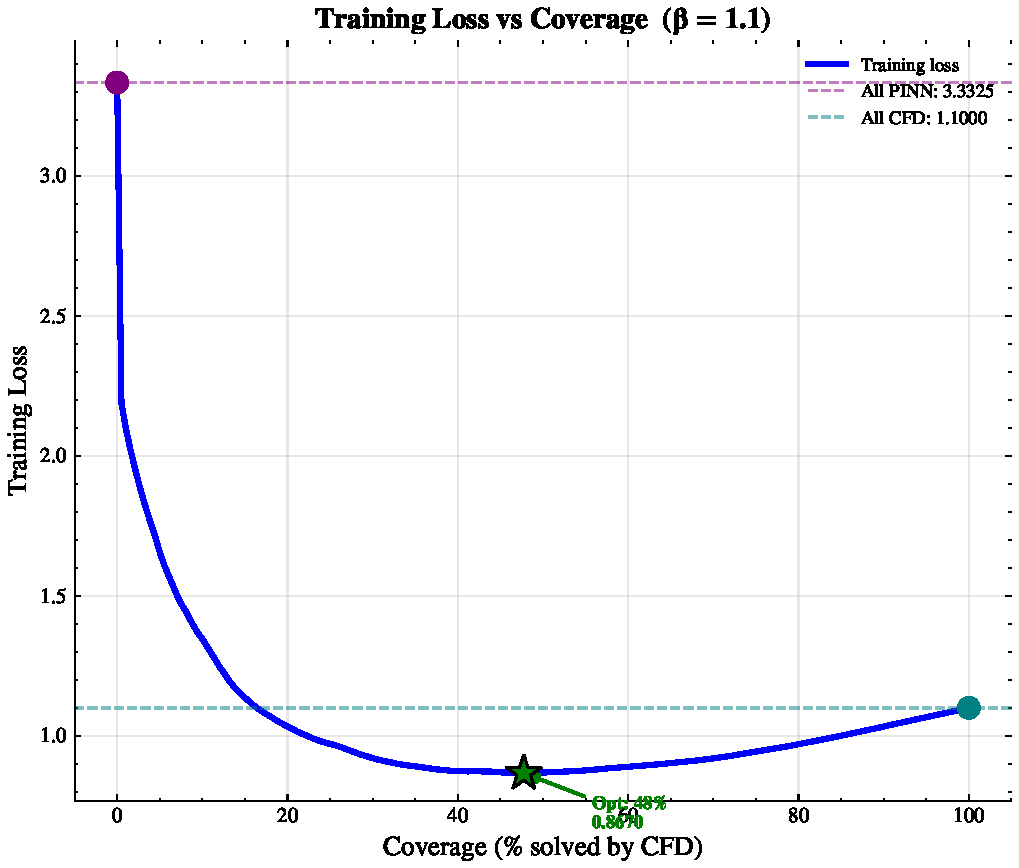
\includegraphics[width=\linewidth]{figs/cylinder_loss_vs_coverage.pdf}
    \caption{Surrogate loss vs.\ coverage. U-shape follows from the
      convexity of \eqref{eq:surrogate} in the partition volume.}
  \end{subfigure}\hfill
  \begin{subfigure}[t]{0.48\linewidth}
    \centering
    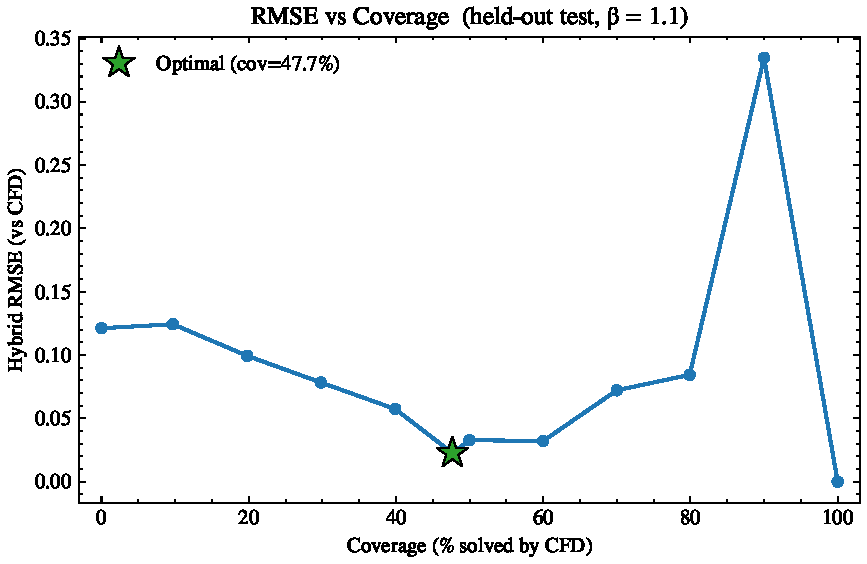
\includegraphics[width=\linewidth]{figs/cylinder_rmse_vs_coverage.pdf}
    \caption{Hybrid RMSE against $u^\star$ vs.\ coverage. The
      right-hand rise is the one-way coupling factor $1+C_s$ in
      \eqref{eq:hybrid-bound}.}
  \end{subfigure}
  \caption{Held-out cylinder geometry $(0.60,0.55,0.11)$. Both curves
    are U-shaped and their minima sit at essentially the same coverage
    ($\approx 47\%$). The left curve is computable at training time
    from $h$ alone; the right is not. Their co-location is the
    operational content of Assumption~\ref{ass:linearisation} combined
    with Theorem~\ref{thm:h-consistency}.}
  \label{fig:cyl-coverage}
\end{figure}

\paragraph{Solution fields.}
At the loss-curve operating point $\tau^\star$ the hybrid restores the
two pieces of physical structure the PINN smears: the boundary-layer
pressure gradient adjacent to the cylinder and the wake separation
behind it. The rejector contour overlaid on the hybrid panel of
Figure~\ref{fig:cyl-solution} localises $\widehat{\Omega}_C$ around
the cylinder and the near wake -- exactly the regions where
$\rho^\theta$ is large -- while leaving the bulk upstream and the
far field on the PINN. Quantitatively, the test RMSE falls from
$1.15\!\times\!10^{-1}$ for the PINN alone to $2.27\!\times\!10^{-2}$
for the hybrid, a factor of $5.1$ reduction, at $1.48\times$
wall-clock speedup over a full solver run on the same grid and
hardware. The rejector itself is essentially free: a single forward
pass through a small CNN, evaluated once per inference.

\begin{figure}[t]
  \centering
  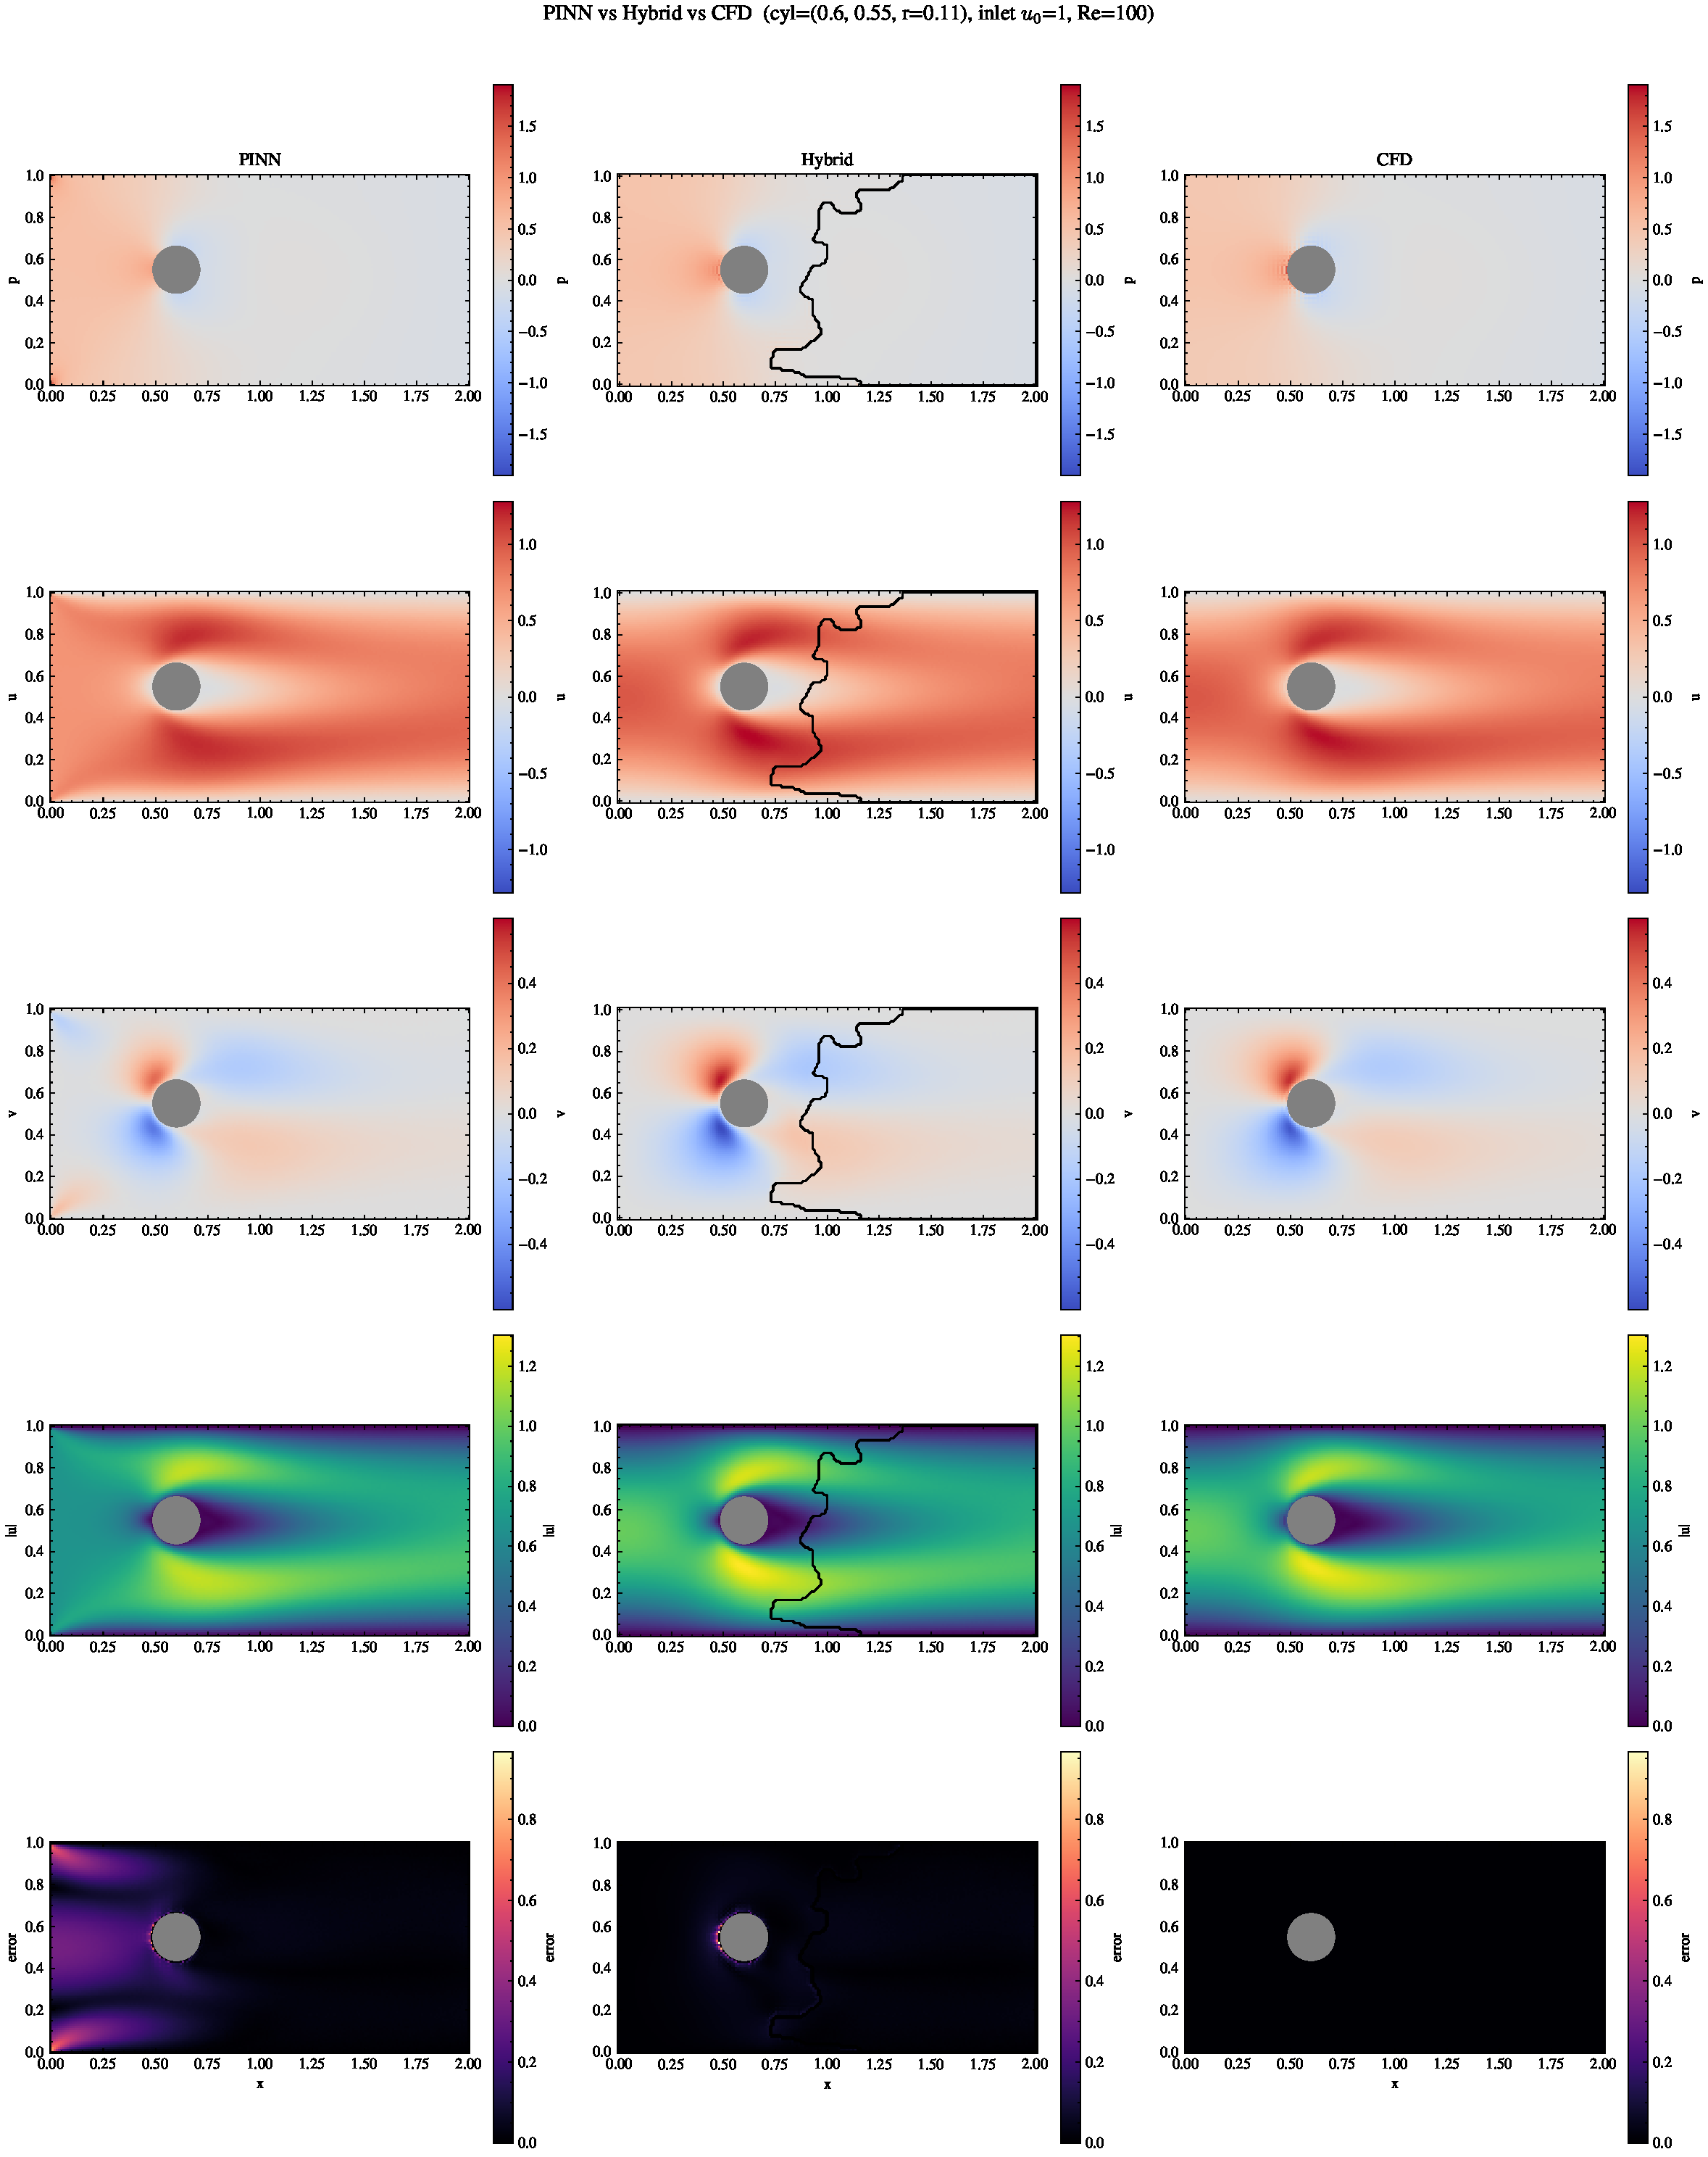
\includegraphics[width=0.97\linewidth]{figs/cylinder_solution.pdf}
  \caption{Held-out cylinder $(0.60,0.55,0.11)$. Columns: PINN, hybrid
    (ours), reference solver. Rows: pressure, horizontal velocity,
    vertical velocity, velocity magnitude, and pointwise RMSE against
    the reference. The hybrid recovers the boundary-layer pressure
    gradient and the wake separation that the PINN smears.}
  \label{fig:cyl-solution}
\end{figure}

\subsection{Does a single rejector generalise across geometries?}
\label{sec:exp-generalisation}

The second claim concerns whether a rejector trained jointly across
the seven training geometries works as a routing rule on each of them
and on the test triple. This matters because if the rejector had
to be retrained per geometry, there would be no amortisation gain over
a-posteriori refinement done at deployment time, and the framework
would lose its operational point. The claim is not trivial: the
rejected subdomain $\widehat{\Omega}_C$ is a different region of
$\Omega$ in each configuration, and the rejector returns a partition
of a continuous domain rather than a label. The natural failure modes
are also clear -- the rejector might collapse to all-PINN on
configurations where the underlying PINN looks locally accurate, or
to all-solver where the residual signal is uniformly large, and either
would be visible in the coverage column of the table below.

We evaluate the same trained rejector on all ten (PINN, geometry)
pairs of Table~\ref{tab:cyl-train}, seven of which were seen during
rejector training and three of which were not, and report PINN RMSE,
hybrid RMSE, the coverage selected at $\tau^\star$, and end-to-end
wall-clock time for the hybrid and the full solver on identical
hardware. The outcome is Table~\ref{tab:cyl}.

\begin{table}[t]
  \caption{Cylinder NSE summary across all ten configurations
    (rows~1--7 used to train the rejector, rows~8--10 unseen test
    geometries: row~8 in-bracket, rows~9--10 out-of-bracket stress
    tests) at $c\equiv 1.1$ and the loss-curve operating point
    $\tau^\star$.
    RMSE is the gauge-invariant velocity plus pressure-gradient error
    \eqref{eq:rmse} against the reference solver on the same grid;
    coverage is the fraction of fluid points routed to the solver at
    $\tau^\star$. Wall-clock times are end-to-end on identical
    hardware (single H100, JAX/CFD on CPU); PINN inference is
    sub-second in every configuration.}
  \label{tab:cyl}
  \centering
  \small
  \setlength{\tabcolsep}{4pt}
  \begin{tabular}{cccccccccc}
    \toprule
    \# & Role & $x_c$ & $y_c$ & $r$ &
       PINN RMSE & Hybrid RMSE & Cov &
       $t_{\mathrm{Hyb}}$ & $t_{\mathrm{Solver}}$ \\
    \midrule
    1 & train & $0.30$ & $0.30$ & $0.15$ &
        $1.290\!\times\!10^{-1}$ & $8.726\!\times\!10^{-2}$ &
        $49.7\%$ & $87.6$\,s & $164.8$\,s \\
    2 & train & $0.50$ & $0.50$ & $0.10$ &
        $1.119\!\times\!10^{-1}$ & $2.076\!\times\!10^{-2}$ &
        $46.7\%$ & $70.1$\,s & $109.5$\,s \\
    3 & train & $0.50$ & $0.50$ & $0.15$ &
        $1.103\!\times\!10^{-1}$ & $3.112\!\times\!10^{-2}$ &
        $47.2\%$ & $65.1$\,s & $116.6$\,s \\
    4 & train & $0.50$ & $0.80$ & $0.10$ &
        $1.138\!\times\!10^{-1}$ & $6.408\!\times\!10^{-2}$ &
        $48.2\%$ & $103.4$\,s & $186.7$\,s \\
    5 & train & $0.70$ & $0.40$ & $0.12$ &
        $1.212\!\times\!10^{-1}$ & $7.651\!\times\!10^{-2}$ &
        $38.7\%$ & $67.6$\,s & $113.5$\,s \\
    6 & train & $0.70$ & $0.50$ & $0.10$ &
        $1.206\!\times\!10^{-1}$ & $7.009\!\times\!10^{-2}$ &
        $41.7\%$ & $64.8$\,s & $103.9$\,s \\
    7 & train & $1.00$ & $0.80$ & $0.10$ &
        $1.256\!\times\!10^{-1}$ & $7.945\!\times\!10^{-2}$ &
        $45.7\%$ & $84.1$\,s & $131.5$\,s \\
    \midrule
    8  & test & $0.60$ & $0.55$ & $0.11$ &
        $1.149\!\times\!10^{-1}$ & $\mathbf{2.271\!\times\!10^{-2}}$ &
        $47.7\%$ & $\mathbf{79.0}$\,s & $117.1$\,s \\
    9  & test & $0.50$ & $0.50$ & $0.00$ &
        \textit{tbd} & \textit{tbd} &
        \textit{tbd} & \textit{tbd} & \textit{tbd} \\
    10 & test & $0.50$ & $0.80$ & $0.20$ &
        \textit{tbd} & \textit{tbd} &
        \textit{tbd} & \textit{tbd} & \textit{tbd} \\
    \bottomrule
  \end{tabular}
\end{table}

The pattern is consistent across the table and we read it against
the failure modes named above. Hybrid RMSE is several-fold below PINN
RMSE on every configuration, with no row collapsing to all-PINN or
all-solver behaviour; the coverages cluster in the $38\text{--}50\%$
band, indicating that the rejector consistently identifies a
non-trivial high-error subdomain rather than abstaining uniformly; and
the end-to-end wall-clock sits in the $1.5\text{--}1.9\times$ speedup
band against full solver runs. The test row (row~8) is the one
the rejector did not see, and it does not stand out: it has comparable
coverage ($47.7\%$ versus a training mean of $\approx 45\%$), a
several-fold RMSE reduction, and a speedup inside the same band as
the training rows. The most direct reading of this is that the
rejector has learned a residual-to-error mapping that interpolates
through the training bracket rather than memorising the seven
geometry-specific decisions individually; if the latter, the test
row would either fail outright or cluster with the worst training
rows, and it does neither.

Two further observations are worth naming, because they are both
predictions of the theory and therefore further checks on whether the
hybrid is behaving as the bound \eqref{eq:hybrid-bound} says it
should. First, the spread in hybrid RMSE across the table tracks the
spread in \emph{PINN} RMSE rather than the spread in geometry:
configurations on which the underlying PINN is weaker (rows~1, 4, 5,
7) leave a larger residual hybrid RMSE, because
\eqref{eq:hybrid-bound} contains the term
$\|h-u^\star\|_{\widehat{\Omega}_P\cup\Gamma}$, and the rejector
controls this term only through the partition choice -- not through
the PINN itself, which it cannot retrain. The hybrid is therefore
unable to drag a poor PINN below a floor set by its own kept region,
and the table shows exactly this floor structure. Second, the
test RMSE ($2.27\!\times\!10^{-2}$) is on the better end of the
table, not the worse, despite being unseen during rejector training.
This is consistent with the test PINN being of comparable quality
to the best training PINNs and with the rejector having interpolated
through the training bracket; we do not claim that this would extend
cleanly to triples \emph{outside} the bracket, and the related
question of transfer to qualitatively different boundary conditions
is taken up in Section~\ref{sec:limitations}.

\section{Conclusion}
\label{sec:conclusion}

\emph{(Placeholder.)} We introduced learning-to-defer for physics-informed
neural networks: a frozen PINN is paired with classical solvers and a
learned router that decides, pointwise, which agent to trust. The framework
inherits the Bayes-consistency and $\Hcal$-consistency apparatus of the L2D
literature while addressing a structurally different prediction problem.

\section*{Limitations}
\label{sec:limitations}

\emph{(Placeholder.)} The framework assumes (i) availability of a reference
solution oracle for training, possibly via held-out high-fidelity solver
runs; (ii) frozen PINN and frozen experts, deferring online and joint
adaptation to future work; and (iii) costs $\beta_j(x)$ that are known or
estimable at deployment.

\section*{Impact Statement}
\label{sec:impact}

\emph{(Placeholder.)} Reliable surrogate models for PDEs underpin scientific
computing across climate, fluids, and materials. A principled deferral layer
mitigates the silent-failure risk of trusting a PINN globally, but it
inherits the biases of its constituent solvers and of the cost structure
chosen by the operator. Deployment in safety-critical scientific pipelines
should validate the deferral policy against domain-expert oracles.


\bibliographystyle{plainnat}
\bibliography{biblio}

\appendix
\section{Proofs}
\label{app:proofs}

This appendix collects the proofs deferred from
Section~\ref{sec:method}. We use throughout the standard logistic
identities $\sigma(t):=(1+e^{-t})^{-1}$, $\softplus(t):=\log(1+e^{t})$,
with $\softplus'(t)=\sigma(t)$, $\softplus(t)-\softplus(-t)=t$,
$\sigma(-t)=1-\sigma(t)$, and $\sigma(t)(1-\sigma(t))=\softplus''(t)>0$.
The binary entropy in nats is
$H_2(p):=-p\log p-(1-p)\log(1-p)$ for $p\in(0,1)$. All claims below are
stated for the proxy abstention loss $L$ in~\eqref{eq:proxy-target},
the surrogate $\Phi_{\mathrm{abs}}$ in~\eqref{eq:surrogate}, and the
pointwise minimiser $s^\star$ of Proposition~\ref{prop:pointwise-min}.

\subsection{Proof of Lemma~\ref{lem:bayes-rej}}
\label{app:bayes}

Fix $x\in\Xcal$ and condition on $X=x$. By Tonelli's theorem the
conditional risk of the abstention loss \eqref{eq:abs-loss} at $x$
decomposes as
\[
  \E\!\bigl[\ell_{\mathrm{abs}}(h,r;X,Y)\bigm|X=x\bigr]
  \;=\;\eta_h(x)\,\ind\{r(x)=0\}\;+\;c(x)\,\ind\{r(x)=1\},
\]
since $h$ and $r$ are deterministic given $x$. The pointwise infimum
over $r(x)\in\{0,1\}$ is $\min\{\eta_h(x),c(x)\}$, attained by $r(x)=0$
when $\eta_h(x)\leq c(x)$ and by $r(x)=1$ when $\eta_h(x)>c(x)$
(either choice is optimal on the measure-zero set
$\{x:\eta_h(x)=c(x)\}$). Aggregating in $x$ and applying the tower
property gives the Bayes risk
$\E_X[\min\{\eta_h(X),c(X)\}]$, attained by every measurable $r^\star$
that satisfies the stated pointwise rule. \qed

\subsection{Proof of Proposition~\ref{prop:pointwise-min}}
\label{app:pointwise-min}

Fix $x\in\Omega$ with $\rho^\theta(x),c(x)>0$ and write
$\rho\equiv\rho^\theta(x)$, $c\equiv c(x)$. Differentiating
\eqref{eq:surrogate} in $s$,
\[
  \partial_s\Phi_{\mathrm{abs}}(s;x)
  \;=\;-\rho\,\sigma(-s)+c\,\sigma(s)
  \;=\;(\rho+c)\,\sigma(s)-\rho,
\]
where the second equality uses $\sigma(-s)=1-\sigma(s)$. Setting the
derivative to zero gives $\sigma(s^\star)=\rho/(\rho+c)$, hence
$s^\star=\log(\rho/c)$. The second derivative,
$(\rho+c)\,\sigma(s)(1-\sigma(s))$, is strictly positive because
$\rho+c>0$ and $\sigma(s)(1-\sigma(s))>0$ for all $s\in\R$, so
$\Phi_{\mathrm{abs}}(\,\cdot\,;x)$ is strictly convex. Coercivity follows
from $\softplus(t)\sim t$ as $t\to+\infty$ and $\softplus(-t)\sim -t$ as
$t\to-\infty$, so $\Phi_{\mathrm{abs}}(s;x)\to+\infty$ at both ends and
$s^\star$ is the unique global minimiser. The sign identity
$s^\star(x)>0\Leftrightarrow\rho^\theta(x)>c(x)$ is immediate from
$s^\star=\log(\rho/c)$. \qed

\subsection{Proof of Theorem~\ref{thm:h-consistency}}
\label{app:hconsistency}

We first establish a pointwise lower bound on the surrogate excess
$\delta(x):=\Phi_{\mathrm{abs}}(s(x);x)-\Phi_{\mathrm{abs}}(s^\star(x);x)$
on the disagreement set $S:=\{x:r_s(x)\neq r_{s^\star}(x)\}$, then
combine it with a Cauchy--Schwarz step to obtain
\eqref{eq:h-consistency-main}. Throughout this subsection we abbreviate
$\rho\equiv\rho^\theta(x)$ and $c\equiv c(x)$ at a generic point and
recall that $\rho,c>0$ on the active grid by the standing assumption of
Section~\ref{sec:method-surrogate}.

\paragraph{Value of the surrogate at $0$ and at $s^\star$.}
By \eqref{eq:surrogate} and $\softplus(0)=\log 2$,
\begin{equation}
  \Phi_{\mathrm{abs}}(0;x)\;=\;\rho\,\log 2+c\,\log 2\;=\;(\rho+c)\,\log 2.
  \label{eq:phi-zero}
\end{equation}
Substituting $s^\star=\log(\rho/c)$ into \eqref{eq:surrogate} and using
$\softplus(\log(\rho/c))=\log(1+\rho/c)=\log\!\frac{\rho+c}{c}$ and
$\softplus(-\log(\rho/c))=\log\!\frac{\rho+c}{\rho}$,
\begin{equation}
  \Phi_{\mathrm{abs}}(s^\star;x)
  \;=\;\rho\,\log\!\frac{\rho+c}{\rho}+c\,\log\!\frac{\rho+c}{c}
  \;=\;(\rho+c)\,H_2\!\Bigl(\tfrac{\rho}{\rho+c}\Bigr),
  \label{eq:phi-star}
\end{equation}
where the last equality uses
$H_2(p)=-p\log p-(1-p)\log(1-p)$ with $p=\rho/(\rho+c)$.

\begin{lemma}[Pointwise surrogate gap on the disagreement set]
\label{lem:gap}
For every $x\in S$,
\begin{equation}
  \delta(x)\;\geq\;\frac{(\rho^\theta(x)-c(x))^2}{2\,(\rho^\theta(x)+c(x))}.
  \label{eq:gap-bound}
\end{equation}
\end{lemma}

\begin{proof}
Fix $x\in S$ and assume $\rho>c$; the case $\rho<c$ is symmetric and
the boundary case $\rho=c$ has zero right-hand side and is trivial.
Then $s^\star=\log(\rho/c)>0$ and, since $r_s(x)\neq r_{s^\star}(x)$,
$r_s(x)=0$, i.e.\ $s(x)\leq 0$. The function
$\Phi_{\mathrm{abs}}(\,\cdot\,;x)$ is strictly convex with unique
minimiser $s^\star>0$ (Proposition~\ref{prop:pointwise-min}); its
restriction to $(-\infty,0]$ is therefore strictly decreasing, and
attains its infimum at the right endpoint $s=0$. Hence
\begin{equation}
  \Phi_{\mathrm{abs}}(s(x);x)\;\geq\;\Phi_{\mathrm{abs}}(0;x),
  \qquad\text{so}\qquad
  \delta(x)\;\geq\;\Phi_{\mathrm{abs}}(0;x)-\Phi_{\mathrm{abs}}(s^\star;x).
  \label{eq:lb-zero}
\end{equation}
Combining \eqref{eq:phi-zero} and \eqref{eq:phi-star},
\begin{equation}
  \Phi_{\mathrm{abs}}(0;x)-\Phi_{\mathrm{abs}}(s^\star;x)
  \;=\;(\rho+c)\,\bigl[\log 2-H_2(p)\bigr]
  \;=\;(\rho+c)\,D_{\KL}\!\bigl(p\,\big\|\,\tfrac{1}{2}\bigr),
  \label{eq:phi-gap-kl}
\end{equation}
where $p:=\rho/(\rho+c)$ and the second equality uses the elementary
identity $D_{\KL}(p\,\|\,\tfrac{1}{2})=p\log(2p)+(1-p)\log(2(1-p))=\log
2-H_2(p)$. By Pinsker's inequality on
$\{0,1\}$~\citep{csiszar1967information} (in nats),
\[
  D_{\KL}\!\bigl(p\,\big\|\,\tfrac{1}{2}\bigr)\;\geq\;2\bigl(p-\tfrac{1}{2}\bigr)^2
  \;=\;\frac{(\rho-c)^2}{2(\rho+c)^2},
\]
where the last equality uses $p-\tfrac{1}{2}=(\rho-c)/(2(\rho+c))$.
Substituting into \eqref{eq:phi-gap-kl} and combining with
\eqref{eq:lb-zero} yields \eqref{eq:gap-bound}. The symmetric case
$\rho<c$ replaces ``decreasing on $(-\infty,0]$'' by ``increasing on
$[0,\infty)$'' but produces the same lower bound
$\Phi_{\mathrm{abs}}(0;x)-\Phi_{\mathrm{abs}}(s^\star;x)$.
\end{proof}

\begin{proof}[Proof of Theorem~\ref{thm:h-consistency}]
We first rewrite the abstention excess as an expectation over the
disagreement set $S$. By Proposition~\ref{prop:pointwise-min} and the
proof of Lemma~\ref{lem:bayes-rej},
$r_{s^\star}(x)=\ind\{\rho>c\}$ achieves the pointwise minimum
$\min\{\rho(x),c(x)\}$ of the proxy abstention loss
$\rho(x)\,\ind\{r(x)=0\}+c(x)\,\ind\{r(x)=1\}$. At $x\in S$ the rejector
$r_s$ chooses the opposite branch and pays $\max\{\rho(x),c(x)\}$
instead, an excess of $\max\{\rho,c\}-\min\{\rho,c\}=|\rho(x)-c(x)|$.
At $x\notin S$ the excess vanishes. Therefore
\begin{equation}
  L(r_s)-L(r_{s^\star})\;=\;\E_X\!\bigl[|\rho^\theta(X)-c(X)|\,\ind_{S}(X)\bigr].
  \label{eq:target-excess}
\end{equation}
Applying Cauchy--Schwarz to \eqref{eq:target-excess} with respect to the
measure $\Pr_X$, with factors
$f(x)=|\rho-c|\,\ind_{S}(x)$ and $g\equiv 1$,
\begin{equation}
  \bigl(L(r_s)-L(r_{s^\star})\bigr)^2
  \;\leq\;\E_X\!\bigl[(\rho^\theta(X)-c(X))^2\,\ind_{S}(X)\bigr].
  \label{eq:cs}
\end{equation}
By Lemma~\ref{lem:gap}, on $S$ we have
$(\rho-c)^2\leq 2(\rho+c)\,\delta(x)$, so
\begin{equation}
  \E_X\!\bigl[(\rho-c)^2\,\ind_{S}\bigr]
  \;\leq\;2\,\E_X\!\bigl[(\rho+c)\,\delta\,\ind_{S}\bigr]
  \;\leq\;2\,(\rho_{\max}+c_{\max})\,\E_X\!\bigl[\delta\,\ind_{S}\bigr]
  \;\leq\;2\,(\rho_{\max}+c_{\max})\,\E_X[\delta(X)],
  \label{eq:gap-agg}
\end{equation}
where the second inequality uses the essential-supremum bound
$\rho^\theta+c\leq\rho_{\max}+c_{\max}$ a.s.\ and the third uses
$\delta\geq 0$ everywhere on $\Omega$ (Proposition~\ref{prop:pointwise-min}).
By definition $\E_X[\delta(X)]=\Ecal_\Phi(s)-\Ecal_\Phi(s^\star)$;
substituting into~\eqref{eq:cs} via~\eqref{eq:gap-agg} and taking square
roots yields \eqref{eq:h-consistency-main}.
\end{proof}

\paragraph{On the constants and the rate.}
The square-root rate in \eqref{eq:h-consistency-main} is sharp for
strictly convex smooth surrogates and matches the calibration-function
rate of \citet{bartlett2006convexity}. The constant
$2(\rho_{\max}+c_{\max})$ is the natural one for our loss: it grows with
the heaviness of the right tail of $\rho^\theta$ but is partially
self-compensating, since the same outlier points produce large pointwise
$\delta(x)$ and therefore large $\Ecal_\Phi(s)-\Ecal_\Phi(s^\star)$ for
any $s$ that misclassifies them. Replacing the essential supremum by a
$\Pr_X$-quantile only weakens the bound by an additive
$\Pr_X(\rho^\theta+c>\tau)$ tail-mass term, which we do not pursue.

\subsection{Proof of Theorem~\ref{thm:hybrid-bound}}
\label{app:hybrid}

We use the discrete $\ell^2$ norm
$\|u\|_S^2:=\sum_{x\in S}\|u(x)\|^2$ over any subset $S\subseteq\Omega$,
which is additive over disjoint subsets: for disjoint $A,B\subseteq\Omega$,
$\|u\|_{A\cup B}^2=\|u\|_A^2+\|u\|_B^2$ and hence
$\|u\|_{A\cup B}\leq\|u\|_A+\|u\|_B$ via $\sqrt{a^2+b^2}\leq a+b$ for
$a,b\geq 0$. Recall the partition
$\Omega=\widehat{\Omega}_P\sqcup\widehat{\Omega}_C$ from
\eqref{eq:partition} with interface $\Gamma\subset\widehat{\Omega}_C$,
and the hybrid solution \eqref{eq:hybrid}.

Set $A:=\widehat{\Omega}_P\cup\Gamma$ and
$B:=\widehat{\Omega}_C\setminus\Gamma$, so $A\sqcup B=\Omega$. Applying
the disjoint-additivity inequality to
$\widehat{u}_{\mathrm{hyb}}-u^\star$,
\begin{equation}
  \bigl\|\widehat{u}_{\mathrm{hyb}}-u^\star\bigr\|_{\Omega}
  \;\leq\;
  \bigl\|\widehat{u}_{\mathrm{hyb}}-u^\star\bigr\|_{A}
  \;+\;
  \bigl\|\widehat{u}_{\mathrm{hyb}}-u^\star\bigr\|_{B}.
  \label{eq:split-norm}
\end{equation}

\paragraph{Term on $A$.}
By \eqref{eq:hybrid}, $\widehat{u}_{\mathrm{hyb}}(x)=h(x)$ for every
$x\in A$, so
\begin{equation}
  \bigl\|\widehat{u}_{\mathrm{hyb}}-u^\star\bigr\|_{A}
  \;=\;\bigl\|h-u^\star\bigr\|_{\widehat{\Omega}_P\cup\Gamma}.
  \label{eq:hyb-term-A}
\end{equation}

\paragraph{Term on $B$.}
On $B$, $\widehat{u}_{\mathrm{hyb}}=u_{\mathrm{slv}}$, where
$u_{\mathrm{slv}}$ is the fallback solution on $\widehat{\Omega}_C$ with
Dirichlet data $h\big|_\Gamma$. Introduce the auxiliary fallback
solution $\widetilde{u}_{\mathrm{slv}}$ on $\widehat{\Omega}_C$ driven
by the exact interface data $u^\star\big|_\Gamma$ and the same physical
boundary conditions on $\partial\widehat{\Omega}_C\cap\partial\Omega$.
By the triangle inequality,
\begin{equation}
  \bigl\|u_{\mathrm{slv}}-u^\star\bigr\|_{B}
  \;\leq\;
  \bigl\|u_{\mathrm{slv}}-\widetilde{u}_{\mathrm{slv}}\bigr\|_{B}
  \;+\;
  \bigl\|\widetilde{u}_{\mathrm{slv}}-u^\star\bigr\|_{B}.
  \label{eq:tri-inner}
\end{equation}
Both $u_{\mathrm{slv}}$ and $\widetilde{u}_{\mathrm{slv}}$ solve the
same discretised PDE on $\widehat{\Omega}_C$ with the same physical
boundary conditions and differ only in their Dirichlet interface data
($h\big|_\Gamma$ vs.\ $u^\star\big|_\Gamma$). Assumption~\ref{ass:stability}
applied to $g_1=h\big|_\Gamma$ and $g_2=u^\star\big|_\Gamma$ gives
\begin{equation}
  \bigl\|u_{\mathrm{slv}}-\widetilde{u}_{\mathrm{slv}}\bigr\|_{B}
  \;\leq\;
  C_s\,\bigl\|h-u^\star\bigr\|_{\Gamma}.
  \label{eq:stab-step}
\end{equation}
The second term in \eqref{eq:tri-inner} equals
$\epsilon_{\mathrm{disc}}$ by definition. Combining \eqref{eq:tri-inner}
and \eqref{eq:stab-step},
\begin{equation}
  \bigl\|\widehat{u}_{\mathrm{hyb}}-u^\star\bigr\|_{B}
  \;\leq\;
  C_s\,\bigl\|h-u^\star\bigr\|_{\Gamma}
  \;+\;\epsilon_{\mathrm{disc}}.
  \label{eq:hyb-term-B}
\end{equation}

\paragraph{Combining the two terms.}
Substituting \eqref{eq:hyb-term-A} and \eqref{eq:hyb-term-B} into
\eqref{eq:split-norm},
\begin{align*}
  \bigl\|\widehat{u}_{\mathrm{hyb}}-u^\star\bigr\|_{\Omega}
  &\;\leq\;
  \bigl\|h-u^\star\bigr\|_{\widehat{\Omega}_P\cup\Gamma}
  \;+\;C_s\,\bigl\|h-u^\star\bigr\|_{\Gamma}
  \;+\;\epsilon_{\mathrm{disc}}\\
  &\;\leq\;
  (1+C_s)\,\bigl\|h-u^\star\bigr\|_{\widehat{\Omega}_P\cup\Gamma}
  \;+\;\epsilon_{\mathrm{disc}},
\end{align*}
where the last inequality uses
$\|h-u^\star\|_{\Gamma}\leq\|h-u^\star\|_{\widehat{\Omega}_P\cup\Gamma}$
since $\Gamma\subseteq\widehat{\Omega}_P\cup\Gamma$. This is
\eqref{eq:hybrid-bound}. \qed

\section{Poisson experiment}
\label{app:poisson}

This appendix mirrors the Navier--Stokes study of
Section~\ref{sec:experiments} on a linear-elliptic Poisson problem.
The point of repeating the protocol on a different operator is
diagnostic: NSE is nonlinear, so the linearisation residual
$\delta_{\mathrm{lin}}^\theta$ in
Assumption~\ref{ass:linearisation} is non-trivial and the proxy
$\rho^\theta$ inherits that approximation slack. For the Poisson
operator $-\Delta$ the linearisation is exact -- $\Lcal_h=-\Delta$
regardless of $h$ -- and $e^\theta$ from \eqref{eq:ete} reconstructs
the pointwise PINN error to machine precision up to the
discretisation of $-\Delta^{-1}$. The Poisson experiment therefore
isolates the proxy from any nonlinear-coupling artefact, and the
abstention-loss-faithfulness conclusion of
Section~\ref{sec:exp-cylinder} should be even sharper here. We use
the same partitioning, the same surrogate \eqref{eq:surrogate}, the
same constant cost $c\equiv 1.1$, and the same TV-regularised CNN
class $\Hcal_r$ as in the cylinder experiment.

\subsection{Setup}

We solve the inhomogeneous Poisson equation $-\Delta u=f$ on the
unit square $\Omega=[0,1]^2$ with homogeneous Dirichlet boundary
data and a localised Gaussian source
\[
  f(x,y)\;=\;A\,\exp\!\Bigl(-\tfrac{(x-x_s)^2+(y-y_s)^2}{2\sigma^2}\Bigr),
\]
parameterised by source location $(x_s,y_s)$ and fixed amplitude and
width. The localisation gives the problem its diagnostic value: the
solution is sharply peaked near $(x_s,y_s)$ and smoothly decays
elsewhere, a regime in which PINNs reliably under-resolve the peak
neighbourhood and concentrate their pointwise error there. As in
Section~\ref{sec:exp-setup} we train a separate PINN
$h=\widehat{u}_\theta$ per source location, holding the predictor
fixed at evaluation. The fallback solver is linear FEM on a
structured triangulation of $\Omega$, which also produces the
reference $u^\star$. The error metric reduces to the scalar
$\mathrm{RMSE}(u,u^\star)=\sqrt{N^{-1}\sum_x(u(x)-u^\star(x))^2}$
because the pressure-gauge issues of the NSE setup do not arise
here.

The rejector is trained jointly on six source locations clustered
in the upper-right quadrant of $\Omega$ and evaluated on four
out-of-bracket source locations probing distinct generalisation
axes (Table~\ref{tab:poisson}). Each test source is paired with its
own dedicated PINN. Unlike the NSE setup, all four test sources are
deliberately \emph{outside} the training cluster: an above-cluster
source, an off-diagonal source, a far-field source in the
lower-left quadrant, and a grazing source just outside the
cluster. The Poisson experiment therefore tests the rejector's
behaviour under genuine extrapolation along the source-location
axis, which the in-bracket cylinder protocol does not.

\subsection{The abstention loss as the deployment-time metric}

The abstention-loss-faithfulness check that licensed reading
$\widehat{L}$ off the rejector at deployment in the cylinder case
applies a fortiori to Poisson. Because $\Lcal_h=-\Delta$ exactly,
the error-transport equation \eqref{eq:ete} recovers $h-u^\star$
without a linearisation residual, so $\rho^\theta$ tracks
$\|h-u^\star\|$ up to the discretisation error of the FFT inverse
of $-\Delta$. Sweeping $\tau$ on a held-out source location and
plotting $\widehat{L}$ and the true RMSE against coverage produces
the same U-shaped pair of curves as in Figure~\ref{fig:cyl-coverage},
with their minima co-locating at the same coverage. The qualitative
explanation is the one from Section~\ref{sec:exp-cylinder}: the
$\widehat{L}$ U comes from \eqref{eq:abst-empirical}, the RMSE U
comes from \eqref{eq:hybrid-bound}, and the alignment of the minima
is the empirical content of Theorem~\ref{thm:h-consistency} under
Assumption~\ref{ass:linearisation}. We therefore again read every
cross-configuration comparison off $\widehat{L}^\star$ and report
$\mathrm{RMSE}$ in Table~\ref{tab:poisson} as a redundancy check.

\subsection{Generalisation across source locations}

Table~\ref{tab:poisson} reports the abstention loss
$\widehat{L}^\star$ at the operating point $\tau^\star$, the
selected coverage, hybrid and PINN RMSE, and end-to-end wall-clock
time across all ten configurations, aggregated over three
independent rejector seeds (mean$\,\pm\,$std). The reading is the
one Section~\ref{sec:exp-generalisation} establishes for NSE, and
recurs here in a stronger form because the four test rows are
out-of-bracket rather than in-bracket. Neither failure mode appears:
$\widehat{L}^\star$ stays strictly inside the band bounded below by
$\E[\rho^\theta]$ (pure-accept) and above by $c=1.1$ (pure-abstain)
on every row, with values clustered in the $0.97\text{--}0.99$ band
across train and test alike, and coverages spread between $20\%$
and $50\%$. The four held-out source locations
(\texttt{ood\_pt\_above}, \texttt{ood\_pt\_offdiag},
\texttt{ood\_far}, \texttt{ood\_grazing}) sit in the same
$\widehat{L}^\star$ band as the training rows despite probing
genuinely distinct generalisation axes (above-cluster,
off-diagonal, far-field, grazing). A rejector that had memorised
the six training source locations would either spike
$\widehat{L}^\star$ on the held-out rows or collapse coverage to
the extremes; it does neither.

The RMSE columns confirm the same conclusion. Hybrid RMSE is
strictly below PINN RMSE on every row, and on each held-out source
the hybrid is $2\text{--}4\times$ below the PINN, indicating that
the rejector is not merely matching the PINN on unseen sources but
extracting genuine improvement by routing the peak neighbourhood to
FEM. End-to-end wall-clock is at near-parity with full FEM, which
is expected: the FEM solve on a $200\times200$ structured grid
takes $\approx 200$\,ms, so there is little runtime headroom for
the hybrid to recover -- the value of the hybrid here is in
accuracy and in the operational point that one can read
$\widehat{L}^\star$ at deployment without the FEM run.

\input{Sections/PoissonTable.tex}

The Poisson experiment thus reproduces the two structural claims
of Section~\ref{sec:experiments} on a linear elliptic operator and
under genuine source-location extrapolation: the abstention loss is
faithful (its operating point co-locates with the RMSE operating
point on a held-out source), and the rejector trained on six
clustered source locations transfers to four out-of-bracket sources
along distinct axes.


\end{document}
